\documentclass[12pt,a4paper]{article}
\usepackage[utf8]{inputenc}
\usepackage[czech]{babel}
\usepackage{graphicx}
\usepackage{fancyhdr}
\usepackage{amsmath}
\usepackage{float}
\usepackage[left=2cm,right=2cm,top=2cm,bottom=2cm]{geometry}
% Hyperlinks and PDF bookmarks
\usepackage[hidelinks,unicode,pdfencoding=auto]{hyperref}
\hypersetup{
	pdftitle={Domácí Úkol 00},
	pdfauthor={Jáchym Kouba},
	bookmarksopen=true,
	bookmarksnumbered=true
}

% Page numbering and header/footer setup
\pagestyle{fancy}
\fancyhf{}
\lhead{Jáchym Kouba}
\rhead{22. února 2026}
\cfoot{\thepage}

% Add dot after section numbers
\renewcommand{\thesection}{\arabic{section}.}
\renewcommand{\thesubsection}{\thesection\arabic{subsection}.}

\title{Domácí Úkol 00}
\author{Jáchym Kouba}
\date{22. února 2026}

\begin{document}

\maketitle
\thispagestyle{fancy}

\section{Úvod}

Úkol jsem zpracoval do sešitu a ofotil. Případné grafy, simulink modely, atd. jsem doplnil jako přílohy do 
pdf, jména kapitol odpovídají úkolu.

\section{Fotografie výpočtů}

\begin{figure}[H]
\centering
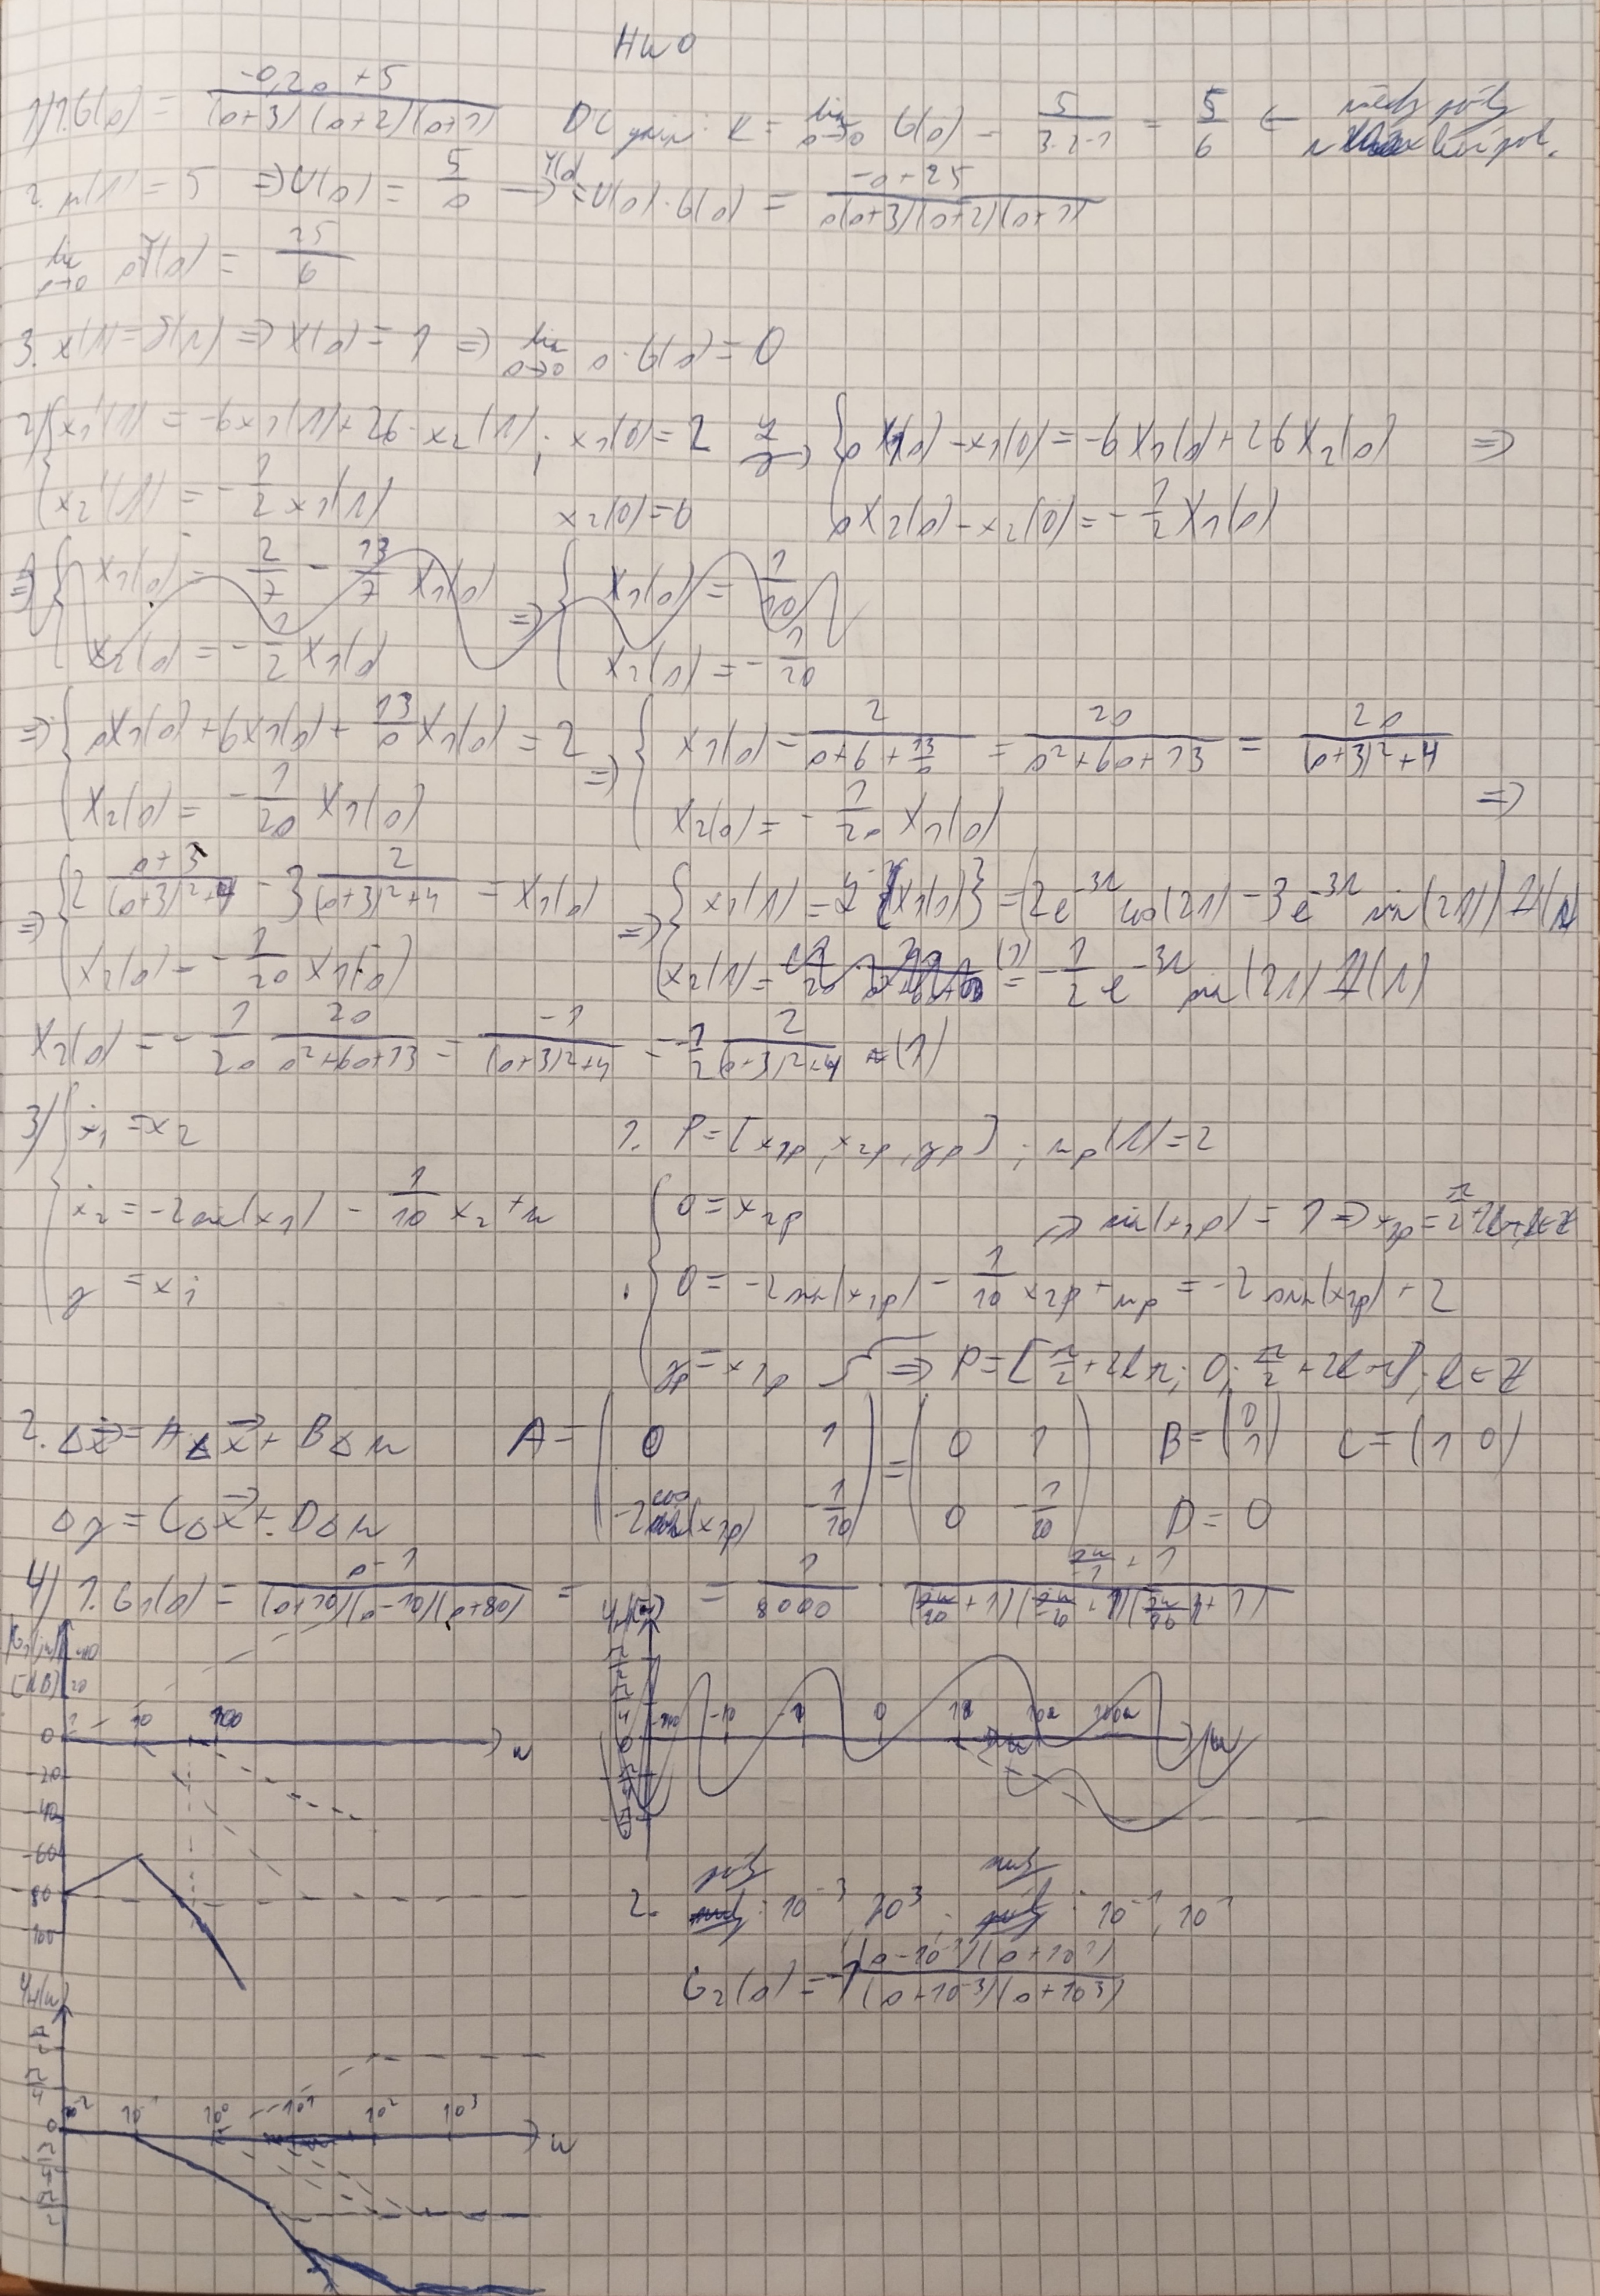
\includegraphics[width=0.8\textwidth]{hw0_1.jpg}
\caption{Výpočty - strana 1}
\label{fig:hw01}
\end{figure}

\begin{figure}[H]
\centering
\includegraphics[width=0.8\textwidth]{hw0_2.jpg}
\caption{Výpočty - strana 2}
\label{fig:hw02}
\end{figure}

\begin{figure}[H]
\centering
\includegraphics[width=0.8\textwidth]{hw0_3.jpg}
\caption{Výpočty - strana 3}
\label{fig:hw03}
\end{figure}

\section{Úkol 02}

\begin{figure}[H]
\centering
\includegraphics[width=0.8\textwidth]{task_02.jpg}
\caption{Úkol 02 - graf}
\label{fig:task02}
\end{figure}

\section{Úkol 03}

\begin{figure}[H]
\centering
\includegraphics[width=0.48\textwidth]{task_03_u1.jpg}\hfill
\includegraphics[width=0.48\textwidth]{task_03_u2.jpg}
\caption{Úkol 03 - Vstupní signály u = 1 (vlevo) a u = 2.0001 (vpravo)}
\label{fig:task03_inputs}
\end{figure}

\begin{figure}[H]
\centering
\includegraphics[width=0.8\textwidth]{task_03_simulink_model.png}
\caption{Úkol 03 - Simulink model}
\label{fig:task03_model}
\end{figure}

\section{Úkol 07}

\begin{figure}[H]
\centering
\includegraphics[width=0.8\textwidth]{task_07_graph_correct.jpg}
\caption{Úkol 07 - Vhodná Ts}
\label{fig:task07_correct}
\end{figure}

\begin{figure}[H]
\centering
\includegraphics[width=0.8\textwidth]{task_07_graph_incorrect.jpg}
\caption{Úkol 07 - Nevhodná Ts}
\label{fig:task07_incorrect}
\end{figure}

\section{Úkol 10}

\begin{figure}[H]
\centering
\includegraphics[width=0.8\textwidth]{task_10_graph.jpg}
\caption{Úkol 10 - Graf}
\label{fig:task10}
\end{figure}

\end{document}
